%author: yjw, 2024-4-1
%\subsection{关键设计}
\subsection{系统需求分析}
\setParDis %设置段间距为 0
%@author: wkt
\begin{enumerate}
  \item 高覆盖率
  \item 高效性快速收敛
  \item 可拓展性
  \item 准确性高
\end{enumerate}
本项目核心目标是将自动模糊测试(Fuzzing)框架迁移到ROS2系统上,并且针对ROS2特性
对测试效率做出改进提升。具体而言,我们试图寻找更多可能的程序输入口,使测试覆盖的
输入可能性尽可能多;尝试构造质量尽可能高的初始种子;寻找更多反馈信息,用于监控被
测程序(即ROS2节点)的内部状态,以更高效地指导对输入的变异;尝试模拟更多ROS2执行
环境,模拟程序可能遇到的各种实际情况。

\subsubsection{通信环境测试}

\begin{figure}[h]
    \centering
    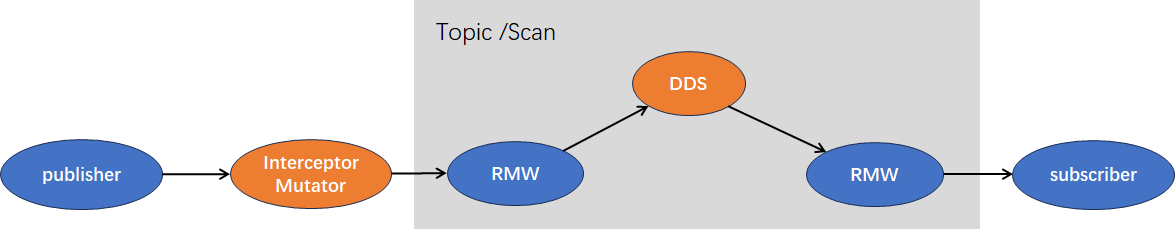
\includegraphics[width=15cm]{fuzz_msg_passing.png}
    \caption{ title}
    \label{pic:fmp}
\end{figure}

\begin{figure}[h]
    \centering
    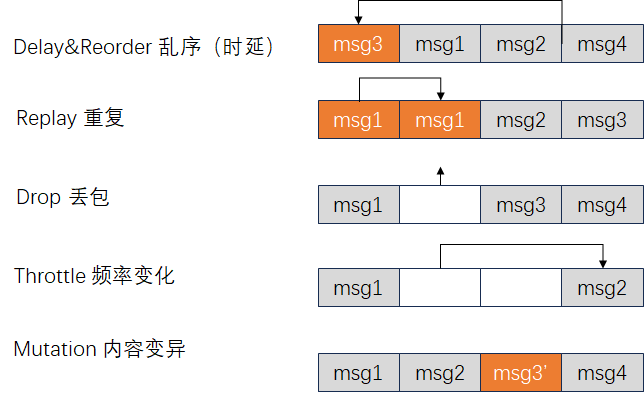
\includegraphics[width=10cm]{fuzz_msg_mutation.png}
    \caption{ title}
    \label{pic:fmm}
\end{figure}

\subsubsection{多维度输入}

\begin{figure}[h]
    \centering
    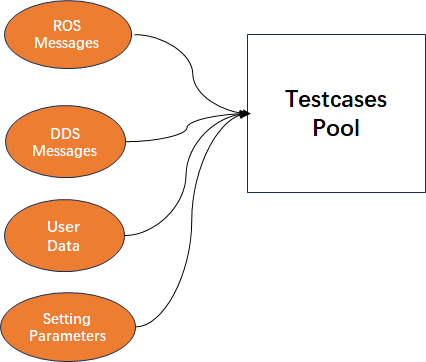
\includegraphics[width=7cm]{fuzz_multi_input.png}
    \caption{ title}
    \label{pic:fmi}
\end{figure}

$^{[2]}$, 

\subsubsection{基于延迟插入的并发漏洞检测}

\begin{figure}[h]
    \centering
    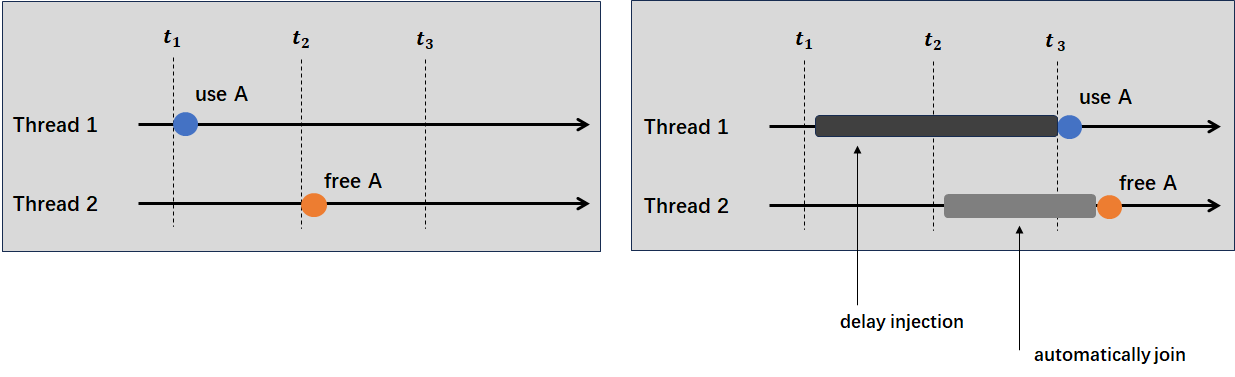
\includegraphics[width=15cm]{fuzz_delay_injection.png}
    \caption{ title}
    \label{pic:fdi}
\end{figure}

\begin{figure}[h]
    \centering
    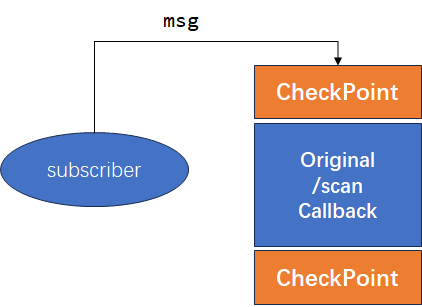
\includegraphics[width=7cm]{fuzz_instrumentation.png}
    \caption{ title}
    \label{pic:fi}
\end{figure}

$^{[1]}$, 

\subsubsection{测试反馈}
\begin{figure}[h]
    \centering
    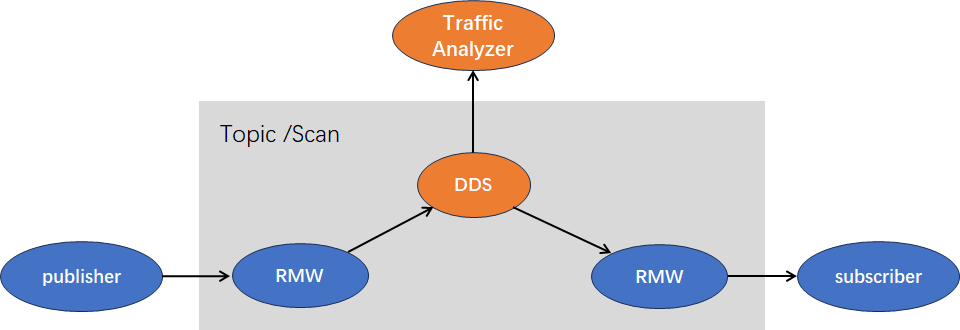
\includegraphics[width=15cm]{fuzz_traffic_monitor.png}
    \caption{ title}
    \label{pic:ftm}
\end{figure}
\subsubsection{测试加速}

